\chapter{本研究における問題定義と仮説}
\label{issue}

本章では, 第~\ref{background}章で述べた背景から, 現状の自動運転システムが目的としている制御方法の問題点を述べる.

\section{最短経路問題}

%% MARK: あとで背景の章に移動

広く一般的に自動運転車が普及すると, 人間による非合理的なブレーキなどの操作がなくなり渋滞が解消すると言われている.
しかし, 渋滞は車線あたりの交通量に比例し, 一般的に自動車の走行ルートを決定する場合, 現在地から目的地までの最短ルートを選択するため
交通需要の高い経路の交通量は変わらず, 自動運転による渋滞解消の因果関係には疑問が残る.
少なくとも同時間帯に同一地点付近の目的地を設定した車が大量にいた場合に特定のルートが混雑が発生することは避けられないと考えられる.
現状のカーナビゲーションシステムなどに搭載されているような渋滞回避機能であっても, 最短経路の周辺の道路に回避され最短経路を選択するには早いもの順になる状態になる.




\begin{figure}[H]
    \centering  % 図を真ん中に配置
    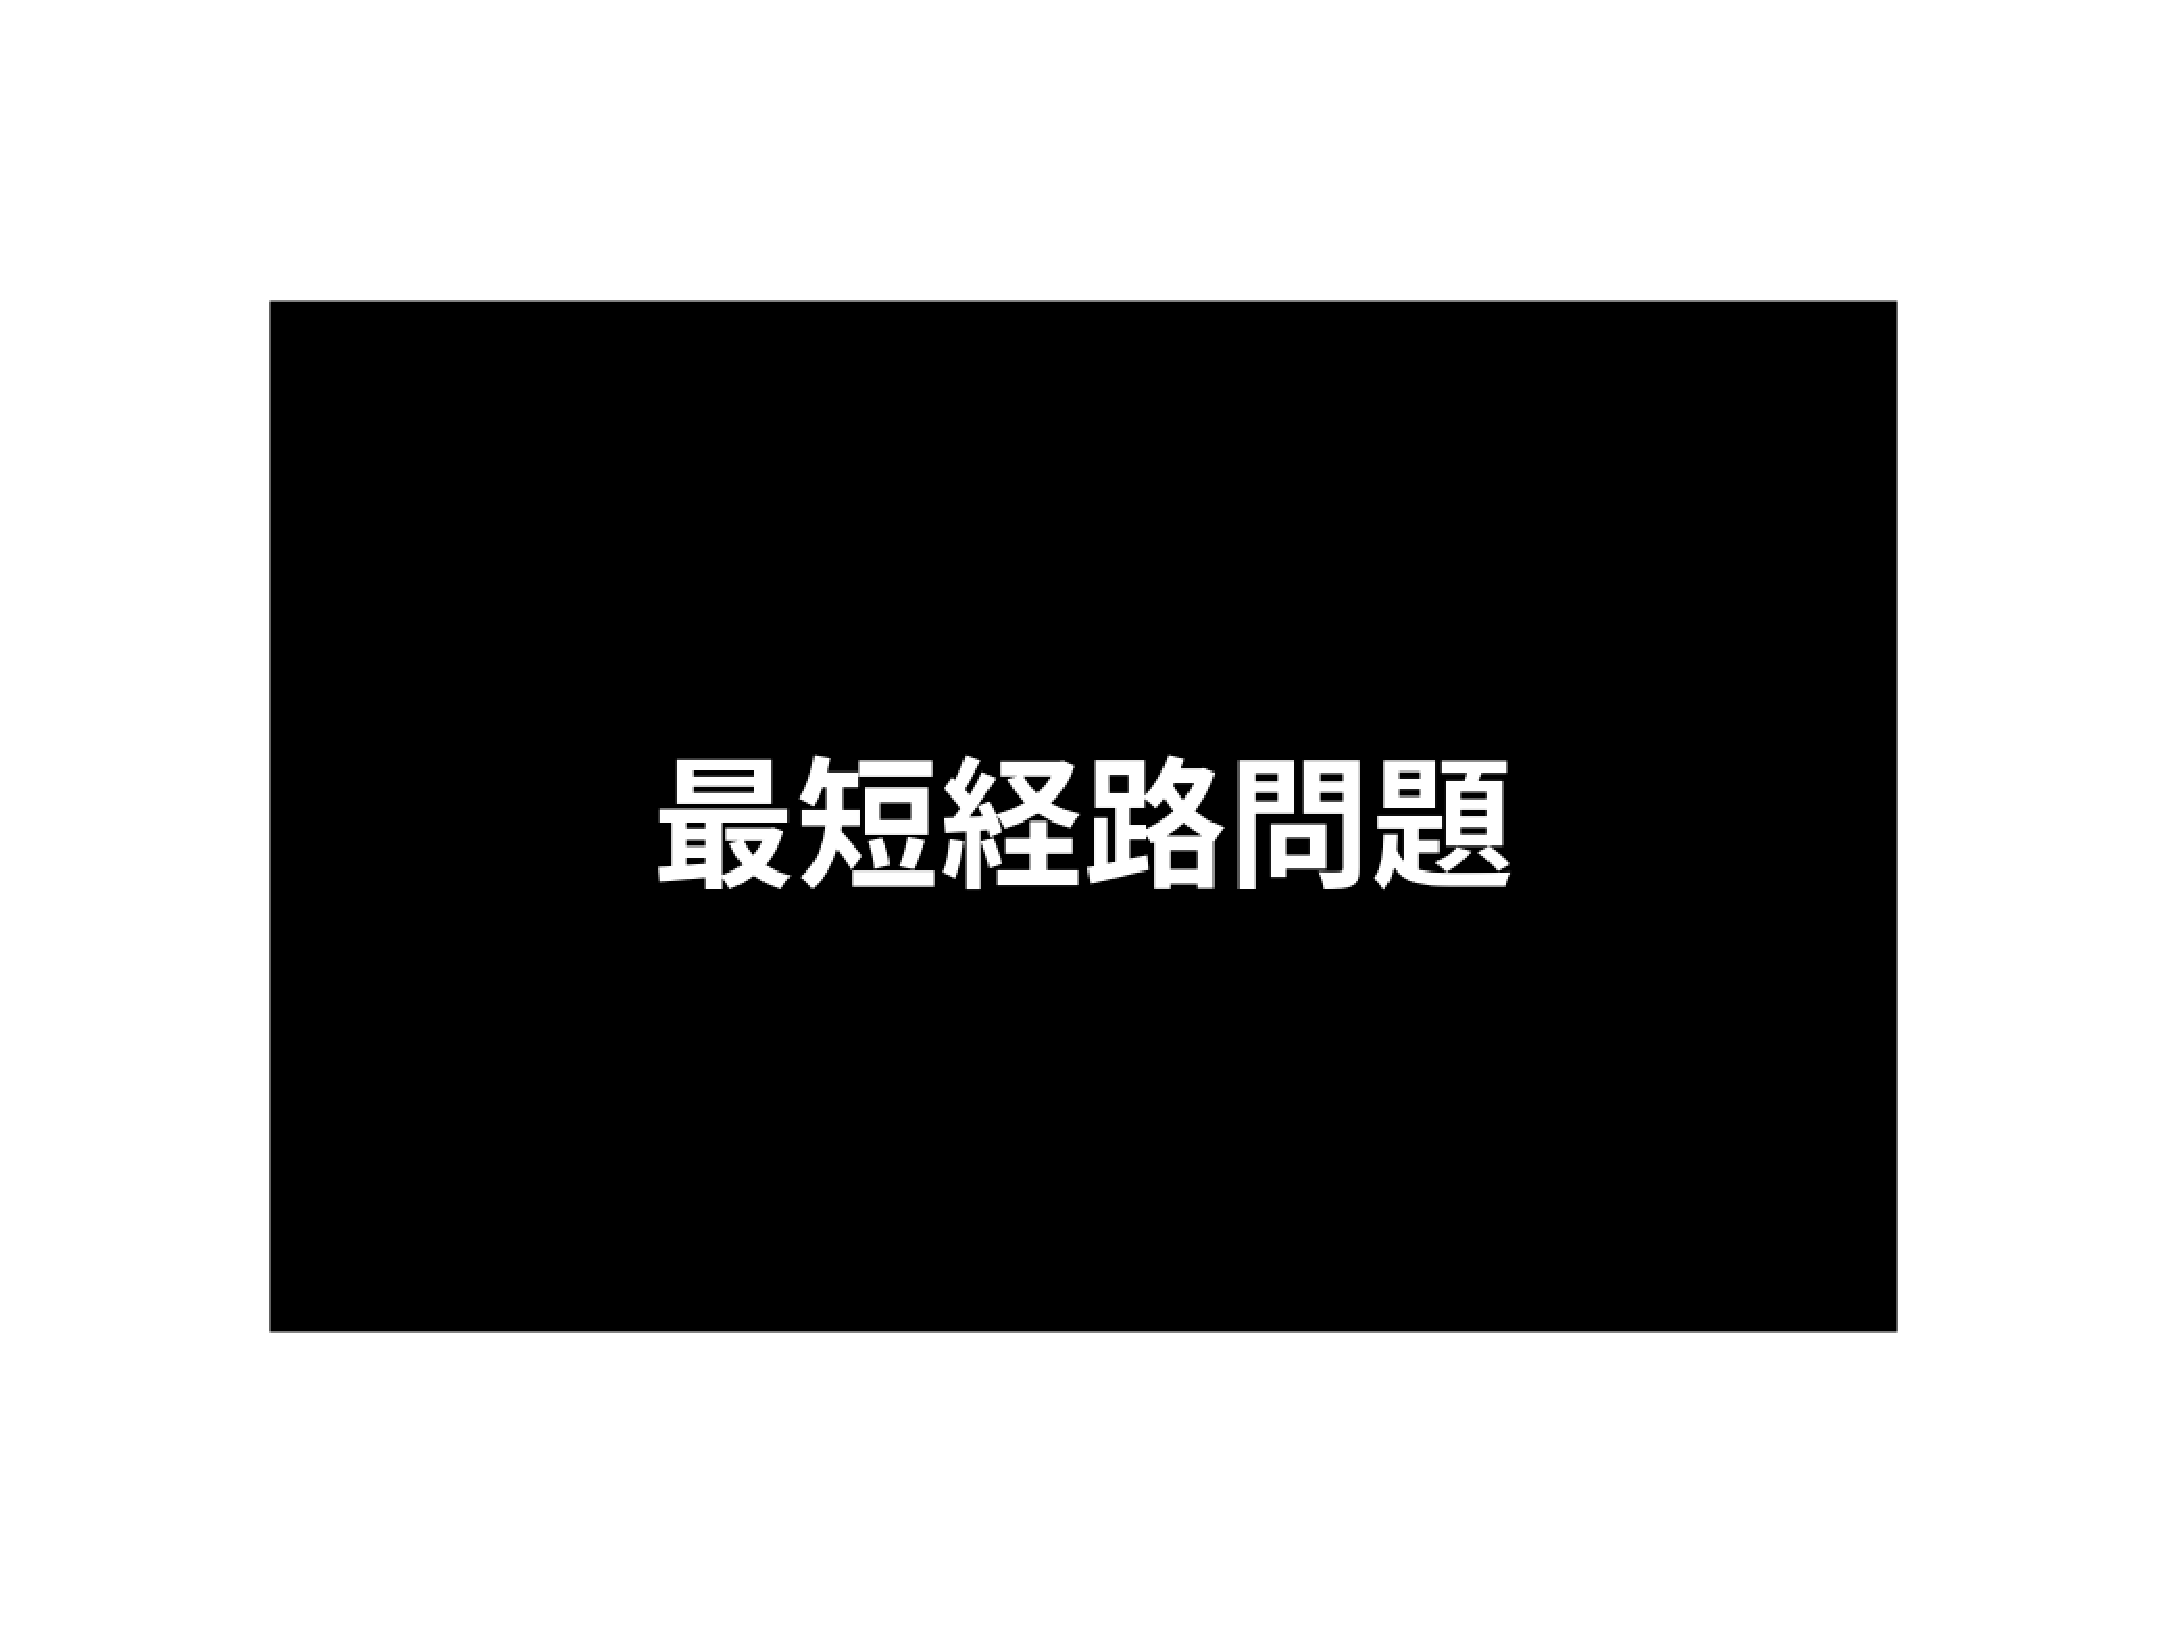
\includegraphics[clip,width = 13.0cm]{assets/shorten_route.eps}
    \caption{最短経路問題}  \label{sample}
\end{figure}

  

\section{本研究における問題定義}

現状の強化学習の問題点を列挙し, 整理する.

\subsection{強化学習によるルート選択}

経路選択に強化学習を応用した事例~\cite{DQNRouteSimple}はすでに存在する. 例えば, 下図のような単純な正方形の升目上の任意の座標にスタート地点とゴール地点を設定し, 最短経路を学習するという物である. 
しかし, 実際の道路網は迷路と比較しても非常に複雑であり沿線との接続や経由地などの要素を考慮す

\textcolor{red}{[ここは修正・加筆必要]}
強化学習を応用した場合の精度は未知数である.

\begin{figure}[H]
    \centering  % 図を真ん中に配置
    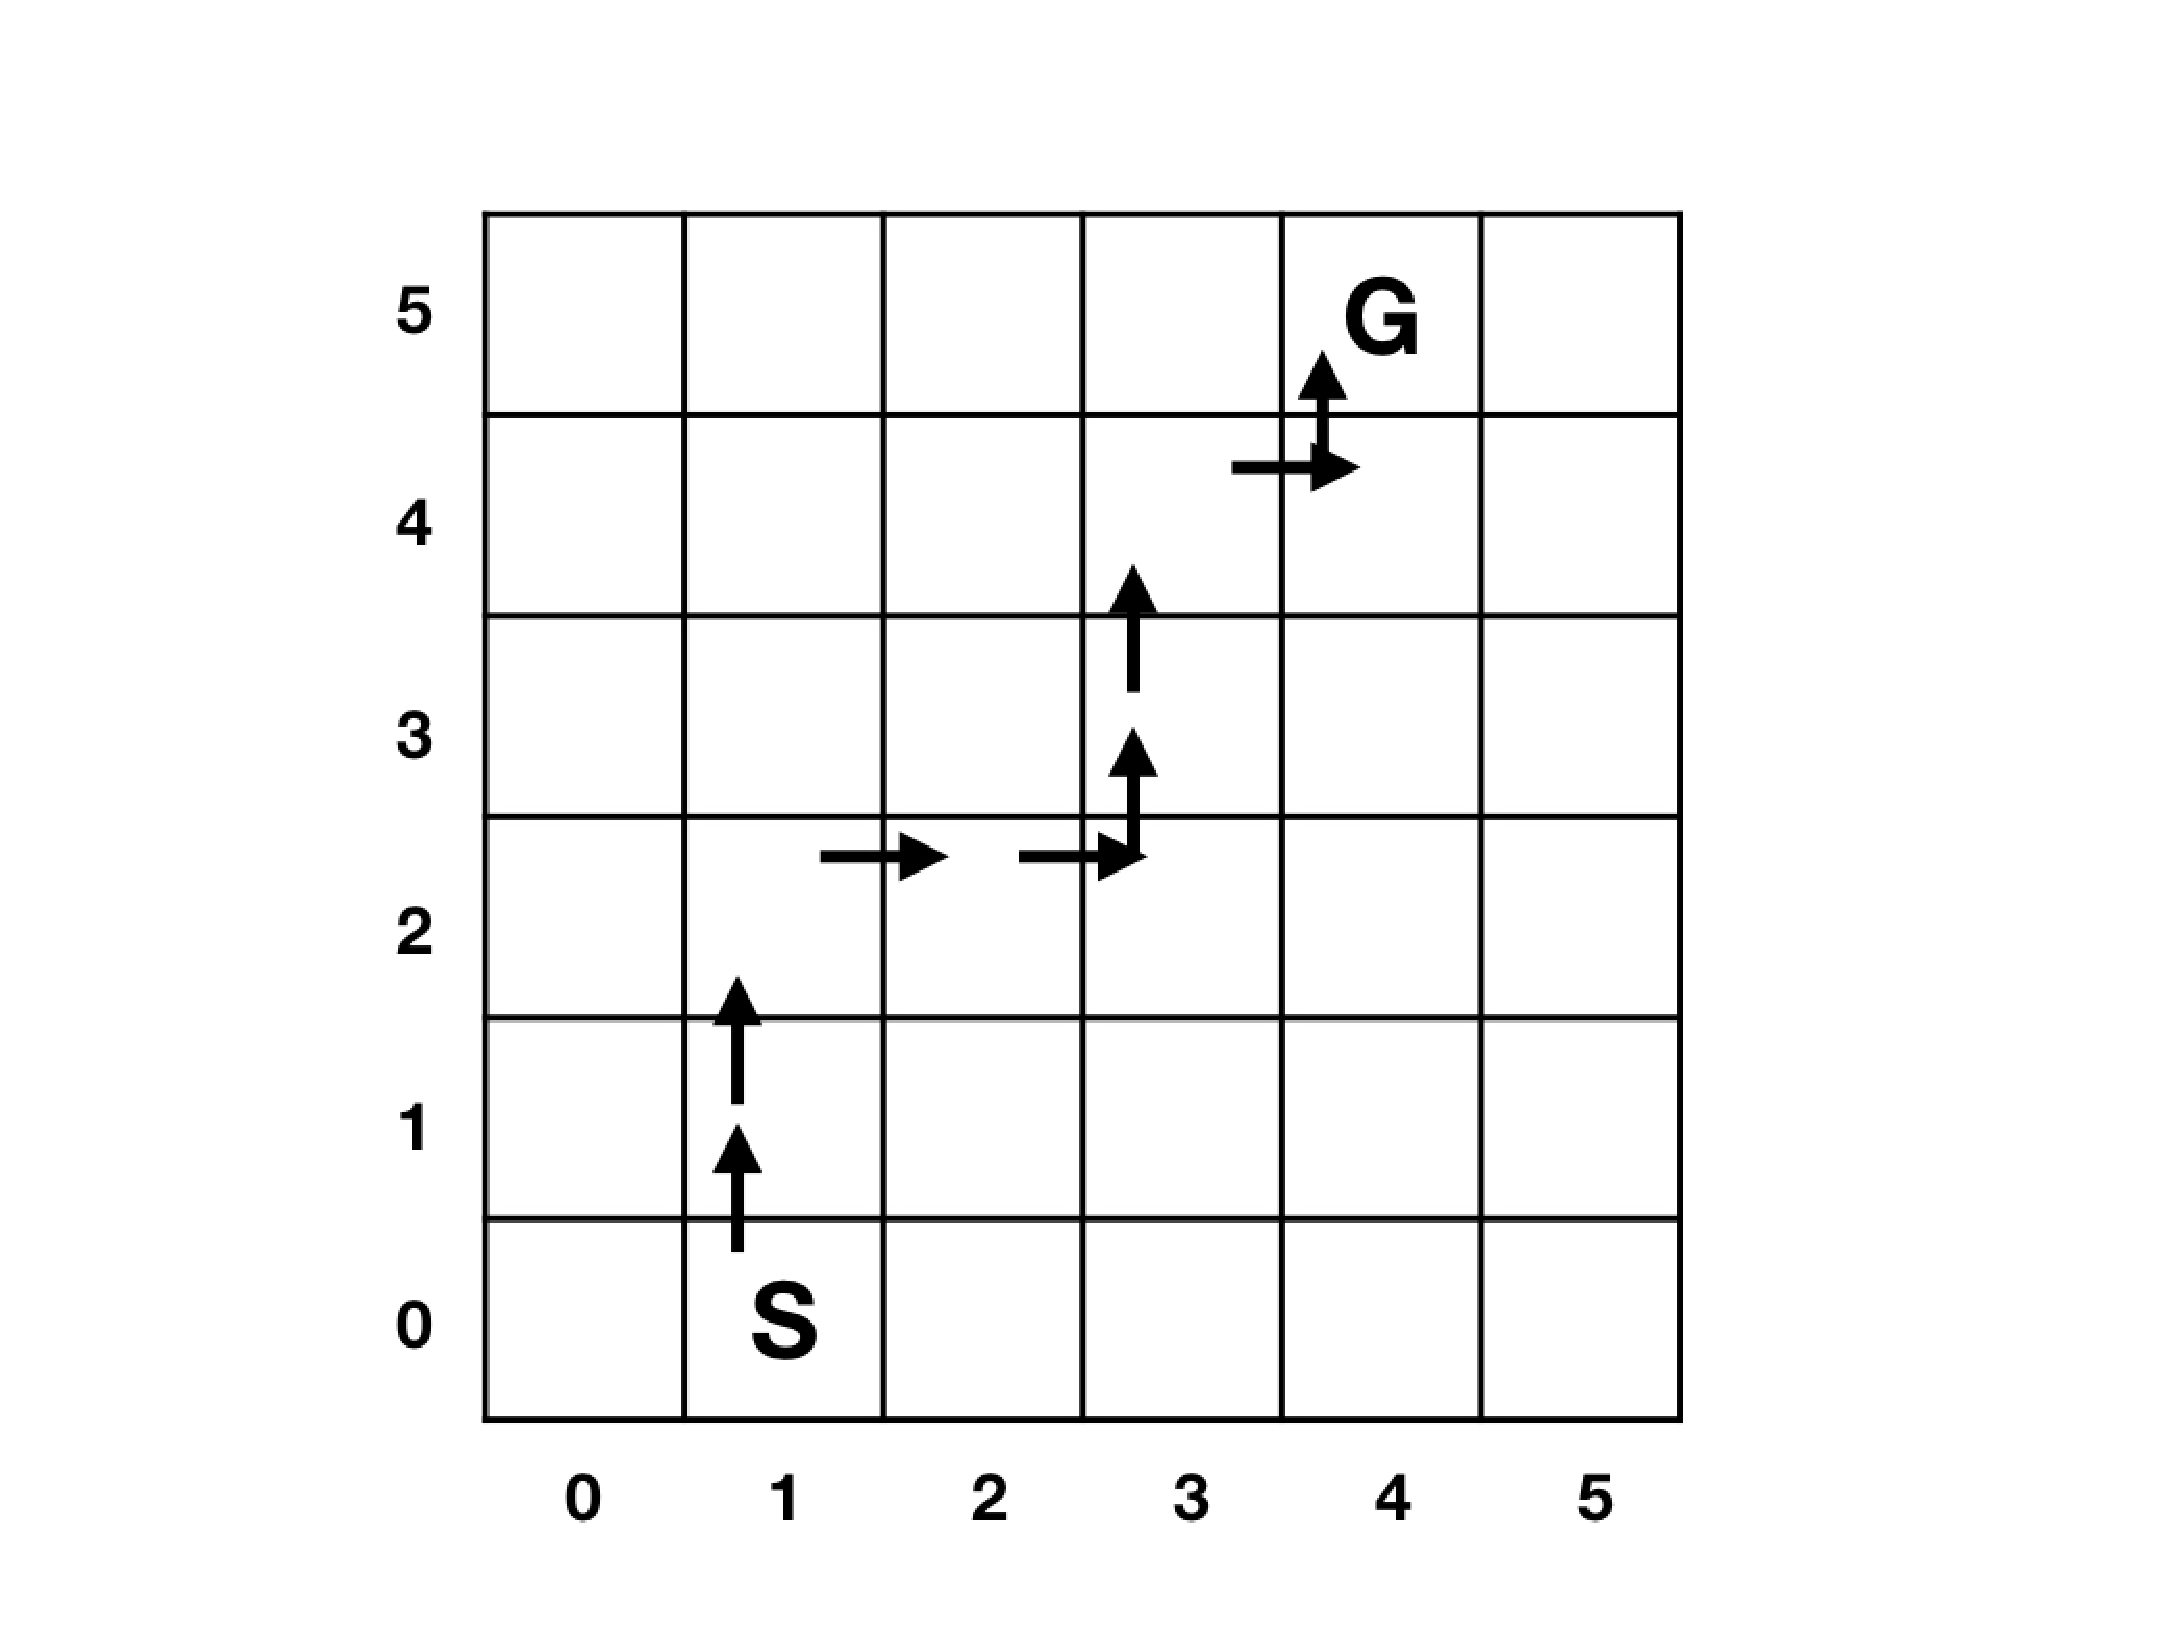
\includegraphics[clip,width = 13.0cm]{assets/rein_simple.eps}
    \caption{強化学習による最短経路検索の結果}  \label{sample}
\end{figure}
  


%% \subsection{ケース策定}   とりあえず仮綴では保留

%% 人間の目的を達成するために  とりあえず仮綴では保留


\section{仮説}

Deep Q Nueral Networkにより学習を繰り返すことで, シミュレーターないでのないでの利用者に最も最適化された経路選択を行うようになると考えた.


%%% Local Variables:
%%% mode: japanese-latex
%%% TeX-master: "./thesis"
%%% End:
